\chapter{Solid-State Chemistry: Bands, Defects and Semiconductors}\label{ch:b3:solid-state}

A solar panel on a roof and the light-emitting diode in a lamp are made of the
same kind of crystal, silicon or a compound of gallium with nitrogen, arsenic
or phosphorus, into which a few impurity atoms per million have been put on
purpose. Their working is set by two things a molecule does not have: bands of
energy levels, with a gap whose width fixes which light a crystal absorbs or
emits, and defects, which carry the charges. This chapter builds the bands
from molecular orbitals, counts the carriers of a \omterm{def:b3:solid-state:classes}{semiconductor}, and treats
missing and misplaced atoms as chemical species with their own equilibria,
down to the \omterm{def:b3:solid-state:ionic-conductor}{solid electrolyte} of the oxygen sensor in a car's exhaust.

\begin{recall}
The Year 1 volume defined crystals, the metallic bond, ionic and covalent
crystals, interstitial sites and alloys, and the Nernst equation; the Year 2
volume the Hückel method and the resonance integral $\beta$.
\Cref{ch:b3:x-ray-diffraction} gave the \omterm{def:b3:x-ray-diffraction:reciprocal}{reciprocal lattice} and
\cref{ch:b3:partition-functions} the \omterm{def:b3:partition-functions:boltzmann}{Boltzmann distribution} and the
\omterm{def:b3:partition-functions:statistical-entropy}{statistical entropy} $S = k\ln W$.
\end{recall}

\begin{omfigure}
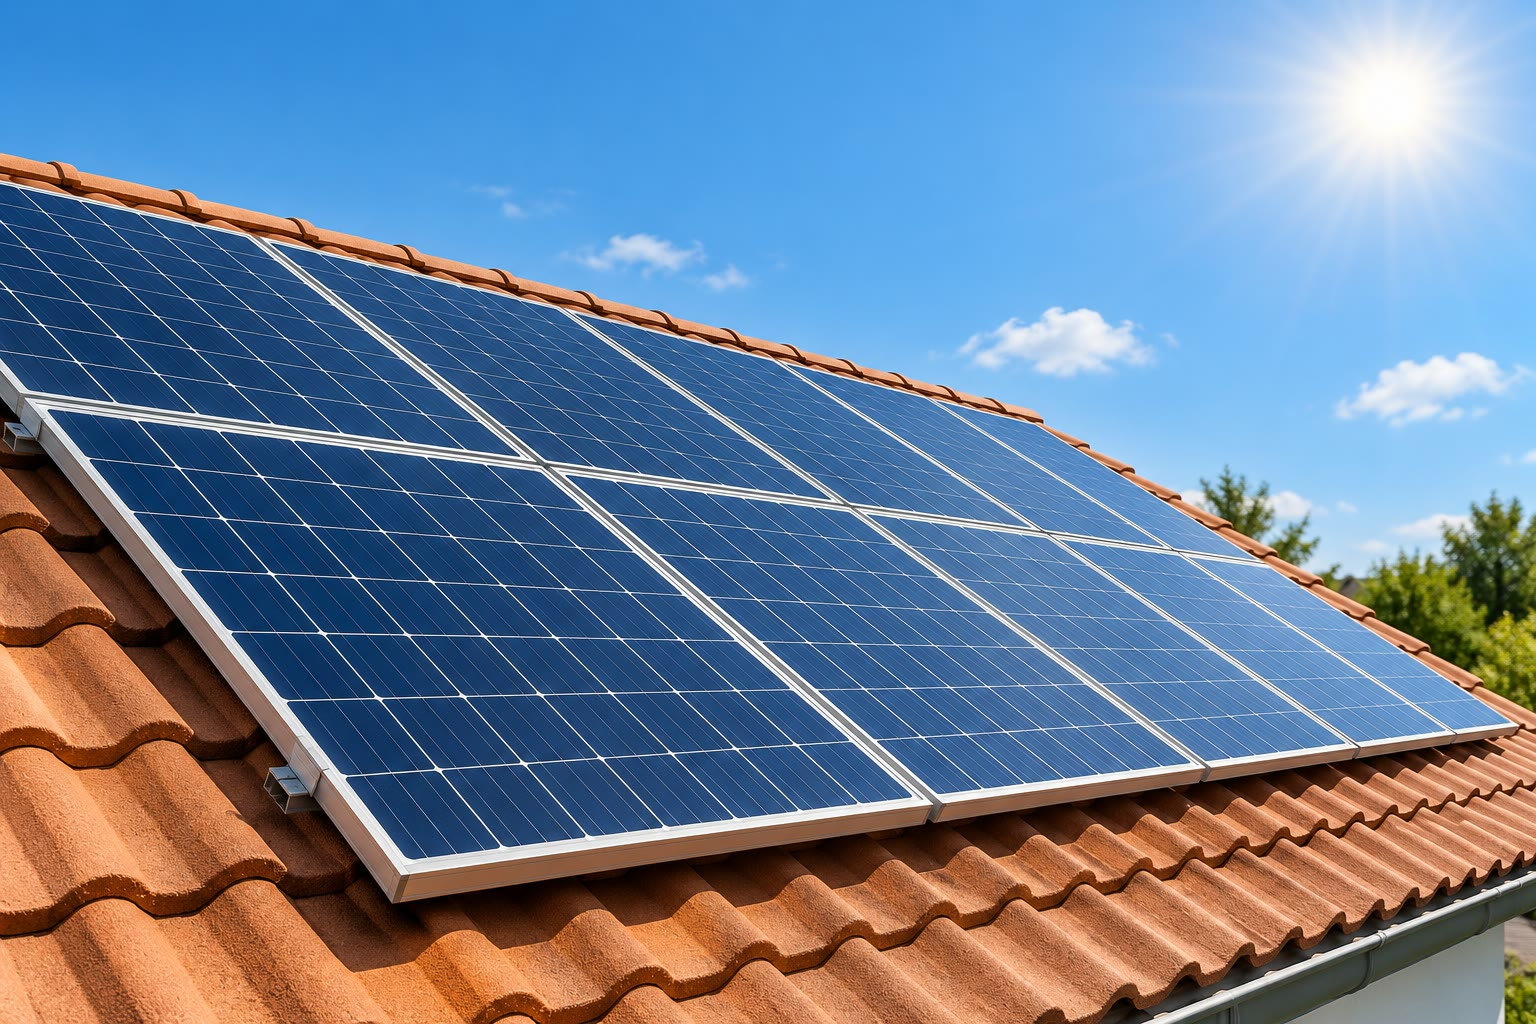
\includegraphics[width=0.6\linewidth]{images/book4/ai/b3-22-solar-panels.jpg}

{\small Solar panels on a tiled roof: each cell is a thin slice of silicon in
which light lifts electrons across a \omterm{def:b3:solid-state:band}{band gap} of about one electronvolt.}
\end{omfigure}

\section{From orbitals to bands}

Take a chain of $N$ identical atoms, each with one s orbital, in the Hückel
approximation: Coulomb integral $\alpha$ on each atom, resonance integral $\beta < 0$
between neighbours, zero otherwise.

\begin{theorem}[Levels of a Hückel chain]\label{thm:b3:solid-state:chain}
The $N$ molecular orbitals of a linear chain of $N$ atoms have energies
\[
  E_k = \alpha + 2\beta\cos\frac{k\pi}{N + 1}, \qquad k = 1, \dots, N,
\]
with coefficients $c_j^{(k)} \propto \sin\bigl(jk\pi/(N + 1)\bigr)$ on atom $j$. As $N \to \infty$ the levels fill the
interval from $\alpha + 2\beta$ to $\alpha - 2\beta$ densely: a band of width $4|\beta|$.
\end{theorem}

\begin{proof}
The secular equations are $\beta c_{j-1} + (\alpha - E)c_j + \beta c_{j+1} = 0$ for $j = 1, \dots, N$, with $c_0 = c_{N+1} = 0$
(no atom there). Try $c_j = \sin(j\theta)$: since $\sin((j - 1)\theta) + \sin((j + 1)\theta) = 2\cos\theta\sin(j\theta)$, each
equation becomes $(\alpha - E + 2\beta\cos\theta)\sin(j\theta) = 0$, so $E = \alpha + 2\beta\cos\theta$. The condition $c_0 = 0$ holds
for every $\theta$, and $c_{N+1} = \sin((N + 1)\theta) = 0$ requires $\theta = k\pi/(N + 1)$; $k = 1, \dots, N$ gives $N$ distinct
levels (the others repeat them or vanish). The lowest and highest are
$\alpha \pm 2\beta\cos(\pi/(N + 1))$, which tend to $\alpha \pm 2\beta$; the spacing between neighbours is at most
$2|\beta|\pi/(N + 1)$, which tends to zero.
\end{proof}

For $N = 2$ the theorem gives $\alpha \pm \beta$, the orbitals of ethene's $\pi$ system; for
$N = 6$ the open-chain hexatriene. In three dimensions the same happens with
every kind of atomic orbital: s orbitals give an s band, p orbitals a p band,
and each band holds $2N$ electrons for $N$ atoms.

\begin{definition}[Bands]\label{def:b3:solid-state:band}
An \emph{energy band}\index{energy band} of a crystal is a continuous range of
allowed one-electron energies, formed from the orbitals of all its atoms. A
\emph{band gap}\index{band gap} $E_g$ is a range of energies with no levels between two
bands. In a \omterm{def:b3:solid-state:classes}{semiconductor} or an \omterm{def:b3:solid-state:classes}{insulator} at zero temperature, the highest
filled band is the \emph{valence band}\index{valence band} and the lowest empty
one the \emph{conduction band}\index{conduction band}.
\end{definition}

\begin{definition}[Density of states and Fermi level]\label{def:b3:solid-state:fermi}
The \emph{density of states}\index{density of states} $g(E)$ is the number of
levels per unit energy (and per atom or per unit volume) near the energy $E$.
The \emph{Fermi level}\index{Fermi level} $E_F$ is the energy at which a level has
probability $1/2$ of being occupied; at zero temperature all levels below it are
filled and all above it empty.
\end{definition}

\begin{omfigure}
\begin{tikzpicture}
\begin{axis}[width=0.78\linewidth, height=6.2cm, xmin=0.3, xmax=7.6, ymin=-2.3, ymax=2.3,
  axis lines=left, xtick={1,2,3,4,5,6.6}, xticklabels={2,4,8,16,64,$\infty$: $g(E)$},
  xlabel={number of atoms $N$}, ylabel={$(E - \alpha)/|\beta|$},
  ytick={-2,-1,0,1,2}, tick label style={font=\small}, label style={font=\small}]
\addplot[only marks, mark=-, mark size=7pt, omDef, thick] table[x=col, y=e] {figdata/out/bachelor-3-band-chain.dat};
\addplot[omThm, thick] table[x expr=6.0+0.55*\thisrow{g}, y=e] {figdata/out/bachelor-3-band-chain-b.dat};
\draw[black!40, dashed] (axis cs:0.3,-2) -- (axis cs:7.6,-2);
\draw[black!40, dashed] (axis cs:0.3,2) -- (axis cs:7.6,2);
\draw[<->, black!60] (axis cs:5.6,-2) -- (axis cs:5.6,2) node[midway, left, font=\scriptsize] {$4|\beta|$};
\end{axis}
\end{tikzpicture}

{\small Hückel levels of chains of 2 to 64 atoms (one short line per level;
with $\beta < 0$ the bonding levels are at the bottom). The levels crowd into a band
between $\alpha + 2\beta$ and $\alpha - 2\beta$; on the right, the \omterm{def:b3:solid-state:fermi}{density of states} of the infinite
chain, largest at the band edges.}
\end{omfigure}

\begin{proposition}[Band filling]\label{prop:b3:solid-state:filling}
A crystal whose highest occupied band is partly filled conducts electricity
like a metal; a crystal whose bands are either full or empty, with a gap
between them, does not conduct at zero temperature.
\end{proposition}

\begin{proof}[Argued]
In an electric field, electrons gain a little energy and momentum: they must
move into empty levels just above the ones they occupy. In a partly filled
band such levels lie immediately above the \omterm{def:b3:solid-state:fermi}{Fermi level}, at no energy cost. In
a full band every level is taken and the next empty one is across the gap;
moreover a full band carries no net current, since for each electron moving
one way another moves the opposite way.
\end{proof}

Sodium, with one 3s electron per atom, half-fills its s band: a metal.
Magnesium, with two, would fill its s band exactly, but the s and p bands
overlap, so it is a metal too. Diamond and silicon have four valence electrons
per atom in orbitals that split into a filled bonding band and an empty
antibonding band, separated by a gap.

\begin{definition}[Semiconductors and insulators]\label{def:b3:solid-state:classes}
A \emph{semiconductor}\index{semiconductor} is a solid with a \omterm{def:b3:solid-state:band}{band gap} small
enough (up to about \qty{3}{eV}) that a measurable number of electrons cross it
at ordinary temperature or after doping; an \emph{insulator}\index{insulator}
has a gap so large that it does not conduct.
\end{definition}

\begin{omfigure}
\begin{tikzpicture}[font=\small]
  \foreach \x/\name in {0/metal, 3.6/semiconductor, 7.2/insulator} {
    \node[font=\small\bfseries] at (\x+0.8,4.3) {\name};
  }
  % metal: one partly filled band
  \fill[omDef!55] (0,0.4) rectangle (1.6,2.0);
  \draw (0,0.4) rectangle (1.6,3.4);
  \draw[omThm, thick] (-0.25,2.0) -- (1.85,2.0) node[right, font=\scriptsize] {$E_F$};
  % semiconductor: small gap
  \fill[omDef!55] (3.6,0.4) rectangle (5.2,1.7);
  \draw (3.6,0.4) rectangle (5.2,1.7);
  \draw (3.6,2.5) rectangle (5.2,3.8);
  \draw[omThm, thick] (3.35,2.1) -- (5.45,2.1) node[right, font=\scriptsize] {$E_F$};
  \draw[<->] (4.4,1.7) -- (4.4,2.5) node[pos=0.8, right, font=\scriptsize] {$E_g$};
  % insulator: large gap
  \fill[omDef!55] (7.2,0.4) rectangle (8.8,1.2);
  \draw (7.2,0.4) rectangle (8.8,1.2);
  \draw (7.2,3.2) rectangle (8.8,4.0);
  \draw[omThm, thick] (6.95,2.2) -- (9.05,2.2) node[right, font=\scriptsize] {$E_F$};
  \draw[<->] (8.0,1.2) -- (8.0,3.2) node[pos=0.75, right, font=\scriptsize] {$E_g$};
  \node[font=\scriptsize, anchor=east] at (3.5,1.05) {valence};
  \node[font=\scriptsize, anchor=east] at (3.5,3.15) {conduction};
  \draw[->] (-0.6,0.2) -- (-0.6,3.9) node[above, font=\scriptsize] {$E$};
\end{tikzpicture}

{\small Band filling at zero temperature (filled levels shaded). A metal has a
partly filled band and its \omterm{def:b3:solid-state:fermi}{Fermi level} inside it; a \omterm{def:b3:solid-state:classes}{semiconductor} and an
\omterm{def:b3:solid-state:classes}{insulator} have a full \omterm{def:b3:solid-state:band}{valence band} and an empty \omterm{def:b3:solid-state:band}{conduction band}, with the \omterm{def:b3:solid-state:fermi}{Fermi
level} in the gap, which is narrow in the first and wide in the second.}
\end{omfigure}

\section{Semiconductors}

\begin{definition}[Carriers]\label{def:b3:solid-state:carriers}
An \emph{intrinsic semiconductor}\index{intrinsic semiconductor} is a pure
\omterm{def:b3:solid-state:classes}{semiconductor}, whose carriers all come from electrons excited across the gap. A
\emph{charge carrier}\index{charge carrier} is a mobile particle that carries
current: an electron in the \omterm{def:b3:solid-state:band}{conduction band}, or a \emph{hole}\index{hole}, an
empty level in the \omterm{def:b3:solid-state:band}{valence band}, which moves like a positive charge.
\end{definition}

\begin{theorem}[Intrinsic carrier concentration]\label{thm:b3:solid-state:intrinsic}
With $N_c$ and $N_v$ the effective densities of states of the conduction and
\omterm{def:b3:solid-state:band}{valence bands} (admitted), the electron and \omterm{def:b3:solid-state:carriers}{hole} concentrations of a \omterm{def:b3:solid-state:classes}{semiconductor}
whose \omterm{def:b3:solid-state:fermi}{Fermi level} is more than a few $kT$ from either band edge are
\[
  n = N_c\,\eu^{-(E_c - E_F)/kT}, \qquad p = N_v\,\eu^{-(E_F - E_v)/kT},
\]
and in an \omterm{def:b3:solid-state:carriers}{intrinsic semiconductor}
\[
  n = p = n_i = \sqrt{N_cN_v}\,\eu^{-E_g/2kT}.
\]
\end{theorem}

\begin{proof}
The occupancy of a level of energy $E$ is $f(E) = 1/(1 + \eu^{(E - E_F)/kT})$. When
$E - E_F \gg kT$, $f \approx \eu^{-(E - E_F)/kT}$, a Boltzmann tail. Summing it over the levels of the \omterm{def:b3:solid-state:band}{conduction
band}, $n = \int g_c(E)\eu^{-(E - E_F)/kT}\,\dd E = \eu^{-(E_c - E_F)/kT}\int g_c(E)\eu^{-(E - E_c)/kT}\,\dd E$, and the last integral is by
definition $N_c$. \omterm{def:b3:solid-state:carriers}{Holes} are empty levels, with probability $1 - f \approx \eu^{-(E_F - E)/kT}$ in the
\omterm{def:b3:solid-state:band}{valence band}; the same steps give $p$. Then $np = N_cN_v\eu^{-(E_c - E_v)/kT} = N_cN_v\eu^{-E_g/kT}$, and in a pure crystal
each excited electron leaves one \omterm{def:b3:solid-state:carriers}{hole}: $n = p$, so $n = \sqrt{np}$.
\end{proof}

\begin{proposition}[Mass-action law]\label{prop:b3:solid-state:mass-action}
In any \omterm{def:b3:solid-state:classes}{semiconductor} at equilibrium, doped or not, $np = n_i^2$.
\end{proposition}

\begin{proof}
The product $np = N_cN_v\eu^{-E_g/kT}$ found in the proof of
\cref{thm:b3:solid-state:intrinsic} does not contain $E_F$: it is the same whatever
sets the \omterm{def:b3:solid-state:fermi}{Fermi level}, and equal to its intrinsic value $n_i^2$. It is the
equilibrium constant of $\text{nothing} \rightleftharpoons \mathrm e^- + \mathrm h^+$, like the ionic product of water.
\end{proof}

\begin{omfigure}
% ledger: eg:Si.E0, eg:Si.a, eg:Si.b, eg:Ge.E0, eg:Ge.a, eg:Ge.b, dos:Si.Nc, dos:Si.Nv, dos:Ge.Nc, dos:Ge.Nv, dop:Si.P
\begin{tikzpicture}
\begin{axis}[name=a, width=0.45\linewidth, height=5.6cm, xmin=1.2, xmax=4.2, ymin=4, ymax=18,
  axis lines=left, xlabel={$1000\,\mathrm K/T$}, ylabel={$\log_{10}(n_i/\unit{cm^{-3}})$},
  tick label style={font=\scriptsize}, label style={font=\small}]
\addplot[omDef, thick] table[x=invT, y=lgSi] {figdata/out/bachelor-3-semiconductor-carriers.dat};
\addplot[omThm, thick] table[x=invT, y=lgGe] {figdata/out/bachelor-3-semiconductor-carriers.dat};
\node[font=\scriptsize, omDef] at (axis cs:3.4,8.3) {Si};
\node[font=\scriptsize, omThm, anchor=south west] at (axis cs:3.4,14.0) {Ge};
\end{axis}
\begin{axis}[at={(a.east)}, anchor=west, xshift=1.7cm, width=0.45\linewidth, height=5.6cm,
  xmin=1, xmax=25, ymin=10, ymax=17, axis lines=left,
  xlabel={$1000\,\mathrm K/T$}, ylabel={$\log_{10}(n/\unit{cm^{-3}})$},
  tick label style={font=\scriptsize}, label style={font=\small}]
\addplot[omDef, thick] table[x=invT, y=lgn] {figdata/out/bachelor-3-semiconductor-carriers-b.dat};
\addplot[black!45, dashed, unbounded coords=jump, restrict y to domain=10:17] table[x=invT, y=lgni] {figdata/out/bachelor-3-semiconductor-carriers-b.dat};
\node[font=\scriptsize, anchor=west] at (axis cs:2.6,16.4) {intrinsic};
\node[font=\scriptsize] at (axis cs:12,15.35) {saturation, $n = N_D$};
\node[font=\scriptsize] at (axis cs:20,13.2) {freeze-out};
\end{axis}
\end{tikzpicture}

{\small Left: intrinsic carrier concentrations of silicon and germanium against
$1/T$ (model with the measured gaps and effective densities of states); the
slopes are close to $-E_g/2k$. Right: electrons in silicon doped with
$\qty{1e15}{cm^{-3}}$ phosphorus: at low temperature the donors hold their electrons
(freeze-out), from about 150 to \qty{500}{K} all are ionised ($n = N_D$), and at high
temperature the intrinsic carriers (dashed, $n_i$) take over.}
\end{omfigure}

\begin{definition}[Direct and indirect gaps]\label{def:b3:solid-state:gap-types}
A \omterm{def:b3:solid-state:classes}{semiconductor} has a \emph{direct band gap}\index{direct band gap} when the
top of its \omterm{def:b3:solid-state:band}{valence band} and the bottom of its \omterm{def:b3:solid-state:band}{conduction band} occur at the same
electron momentum, so that a photon alone can carry an electron across, and an
\emph{indirect band gap}\index{indirect band gap} when they do not, so that the
transition needs a lattice vibration as well.
\end{definition}

% ledger: eg:Si, eg:Ge, eg:GaAs, eg:GaN, eg:GaP
Silicon (\qty{1.12}{eV}) and germanium (\qty{0.66}{eV}) have indirect gaps:
they absorb light well enough in a thick layer, which suits a solar cell, but
emit it very poorly. Gallium arsenide (\qty{1.42}{eV}) and gallium nitride (about
\qty{3.4}{eV}) have direct gaps, the basis of infrared and blue light-emitting
diodes and lasers; gallium phosphide (\qty{2.26}{eV}) is indirect but emits green
light when doped. The colour of many pigments is also a \omterm{def:b3:solid-state:band}{band gap}: a crystal
absorbs all photons with $h\nu > E_g$, so cadmium sulfide, with a gap in the blue,
is yellow.

\begin{definition}[Doping]\label{def:b3:solid-state:doping}
A \emph{dopant}\index{dopant} is a foreign atom put in a \omterm{def:b3:solid-state:classes}{semiconductor} on
purpose, in small amounts, to provide carriers. In an \emph{n-type
semiconductor}\index{n-type semiconductor} the dopant has one more valence
electron than the atom it replaces (phosphorus in silicon) and gives it to the
\omterm{def:b3:solid-state:band}{conduction band} from a \emph{donor level}\index{donor level} just below that
band; in a \emph{p-type semiconductor}\index{p-type semiconductor} it has one
fewer (boron in silicon) and accepts an electron from the \omterm{def:b3:solid-state:band}{valence band} into an
\emph{acceptor level}\index{acceptor level} just above it, leaving a \omterm{def:b3:solid-state:carriers}{hole}.
\end{definition}

\begin{omfigure}
\begin{tikzpicture}[font=\small]
  \foreach \x in {0, 5.2} {
    \fill[omDef!35] (\x,0) rectangle (\x+3.6,1.0);
    \fill[omDef!12] (\x,2.6) rectangle (\x+3.6,3.6);
    \node[font=\scriptsize] at (\x+1.8,0.5) {valence band};
    \node[font=\scriptsize] at (\x+1.8,3.1) {conduction band};
  }
  \foreach \i in {0,...,5} { \draw[omThm, thick] (0.25+\i*0.55,2.35) -- (0.6+\i*0.55,2.35); }
  \node[font=\scriptsize, anchor=west] at (0.1,1.95) {donor levels, \qty{0.045}{eV} below};
  \draw[->, omThm] (0.42,2.42) -- (0.42,2.9);
  \fill[omThm] (0.42,2.95) circle (1.6pt);
  \foreach \i in {0,...,5} { \draw[omMeth, thick] (5.45+\i*0.55,1.25) -- (5.8+\i*0.55,1.25); }
  \node[font=\scriptsize, anchor=west] at (5.3,1.6) {acceptor levels, \qty{0.045}{eV} above};
  \draw[->, omMeth] (5.62,0.7) -- (5.62,1.18);
  \draw[omMeth, fill=white] (5.62,0.62) circle (1.8pt);
  \node[font=\small\bfseries] at (1.8,4.0) {n-type: P in Si};
  \node[font=\small\bfseries] at (7.0,4.0) {p-type: B in Si};
\end{tikzpicture}

{\small Donor and \omterm{def:b3:solid-state:doping}{acceptor levels} in the gap of silicon (gap not to scale: the
\omterm{def:b3:solid-state:doping}{dopant} levels lie about 0.045 eV from the band edges, the gap is 1.12 eV). A
donor gives its electron (dot) to the \omterm{def:b3:solid-state:band}{conduction band}; an acceptor takes one
from the \omterm{def:b3:solid-state:band}{valence band}, leaving a \omterm{def:b3:solid-state:carriers}{hole} (circle).}
\end{omfigure}

% ledger: dop:Si.P, dop:Si.B
The \omterm{def:b3:solid-state:doping}{donor level} of phosphorus lies \qty{0.045}{eV} below the \omterm{def:b3:solid-state:band}{conduction band} of
silicon, less than $2kT$ at room temperature, and boron's \omterm{def:b3:solid-state:doping}{acceptor level} as much
above the \omterm{def:b3:solid-state:band}{valence band}: at \qty{300}{K} nearly every \omterm{def:b3:solid-state:doping}{dopant} is ionised. That is why
one \omterm{def:b3:solid-state:doping}{dopant} atom per $10^7$ silicon atoms ($\qty{5e15}{cm^{-3}}$) raises the
electron concentration a few hundred thousand times.

\begin{method}[Carriers of a doped semiconductor]\label{met:b3:solid-state:doping}
\begin{enumerate}
  \item Check that the temperature is in the saturation range (\omterm{def:b3:solid-state:doping}{dopants} fully
        ionised, $N_D \gg n_i$): then the majority carriers are $n \approx N_D$ (or $p \approx N_A$).
  \item Get the minority carriers from the mass-action law: $p = n_i^2/N_D$.
  \item Place the \omterm{def:b3:solid-state:fermi}{Fermi level}: $E_c - E_F = kT\ln(N_c/n)$, or relative to the intrinsic level,
        $E_F - E_i = kT\ln(n/n_i)$.
  \item If both kinds of \omterm{def:b3:solid-state:doping}{dopant} are present, use the difference $N_D - N_A$.
\end{enumerate}
\end{method}

\begin{definition}[p--n junction]\label{def:b3:solid-state:junction}
A \emph{p--n junction}\index{p--n junction} is the boundary, inside one crystal,
between a p-type and an n-type region.
\end{definition}

At a \omterm{def:b3:solid-state:junction}{p--n junction} electrons diffuse from the n side into the p side and \omterm{def:b3:solid-state:carriers}{holes}
the other way, leaving a thin layer emptied of carriers in which the fixed
ionised \omterm{def:b3:solid-state:doping}{dopants} set up an electric field; at equilibrium the \omterm{def:b3:solid-state:fermi}{Fermi level} is the
same on both sides. A voltage applied one way lowers the barrier and current
flows; the other way it raises it: a diode. In a light-emitting diode, electrons
and \omterm{def:b3:solid-state:carriers}{holes} injected across the junction recombine and emit photons of energy
close to $E_g$; in a solar cell, photons absorbed near the junction make
electron--hole pairs that the field separates, and a current flows in the
external circuit.

\begin{omfigure}
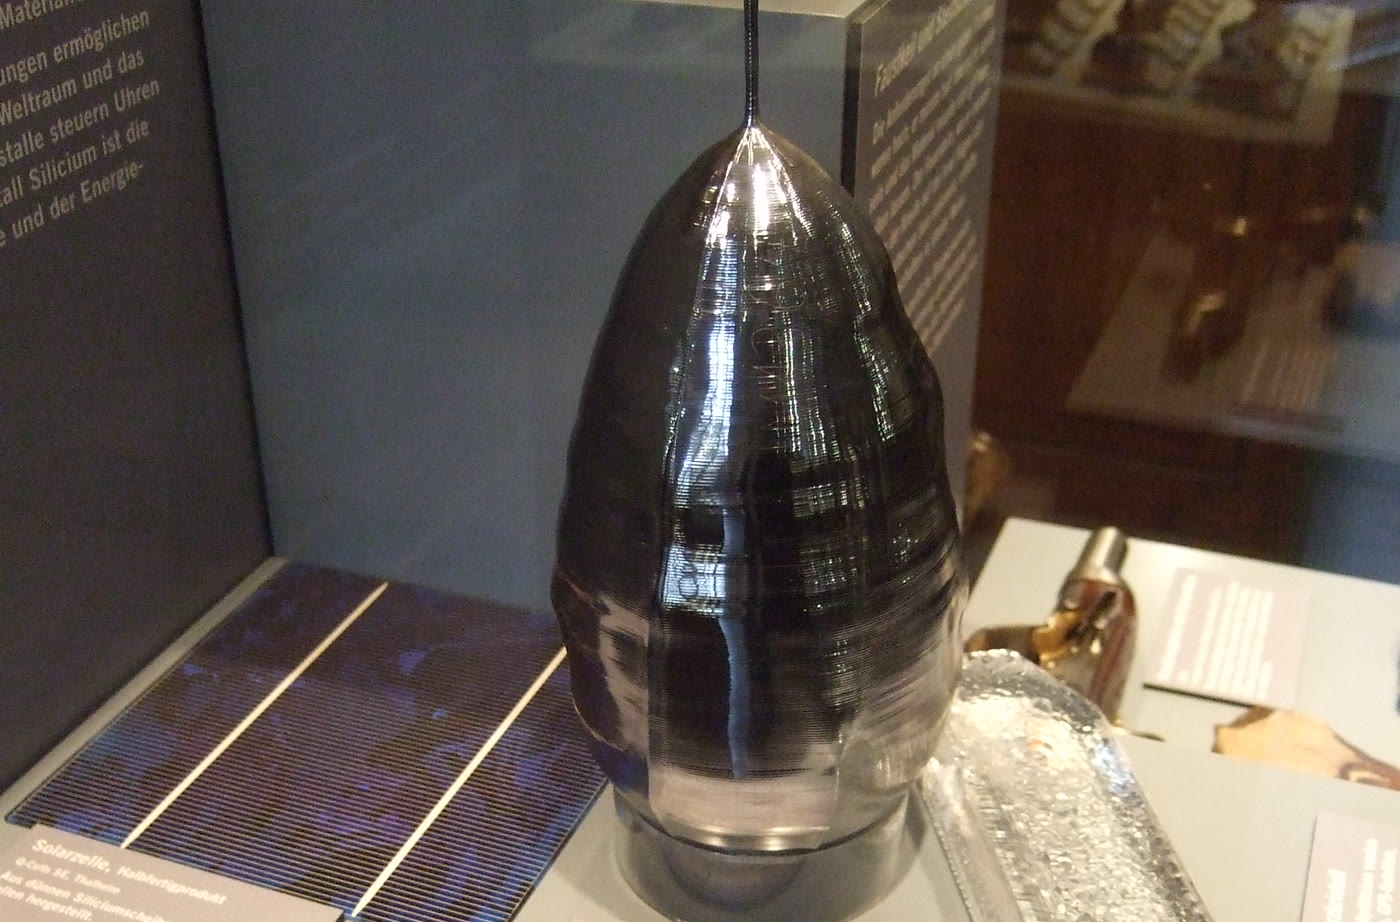
\includegraphics[width=0.5\linewidth]{images/book4/silicon-boule.jpg}

{\small A single crystal of silicon pulled from the melt, shown beside a solar
cell made from a slice of such a crystal. Photograph: Sebastian Wallroth,
public domain.}
\end{omfigure}

\begin{inthelab}[Growing a silicon crystal]
In the Czochralski method, very pure polycrystalline silicon is melted in a
silica crucible under argon, at a little above its melting point, with the
\omterm{def:b3:solid-state:doping}{dopant} added to the melt. A small seed crystal on a rotating rod is dipped into
the melt and slowly raised: silicon crystallises on it with the seed's
orientation, and the rate of pulling and rotation sets the diameter. The boule
is then sawn into wafers less than a millimetre thick. Silane and the doping
gases phosphine and arsine used in later steps are pyrophoric or very toxic,
and are handled only in sealed industrial systems.
\end{inthelab}

\section{Point defects}

\begin{definition}[Point defects]\label{def:b3:solid-state:defects}
A \emph{point defect}\index{point defect} is a departure from the perfect
crystal localised at one site: a vacancy, an interstitial atom, or a foreign
atom. In an ionic crystal, a \emph{Schottky defect}\index{Schottky defect} is a
pair of vacancies, one cation and one anion, the ions having gone to the
surface; a \emph{Frenkel defect}\index{Frenkel defect} is a pair made of a
vacancy and the ion that left it, sitting on an interstitial site.
\end{definition}

\begin{omfigure}
\begin{tikzpicture}[scale=0.62]
  \begin{scope}
  \foreach \i in {0,...,5} \foreach \j in {0,...,4} {
    \pgfmathtruncatemacro{\pty}{mod(\i+\j,2)}
    \ifnum\pty=0 \fill[omDef!70] (\i,\j) circle (0.2); \else \fill[omThm!25] (\i,\j) circle (0.38); \draw[omThm!60] (\i,\j) circle (0.38); \fi
  }
  \fill[white] (2,2) circle (0.45); \draw[dashed] (2,2) circle (0.3);
  \fill[white] (3,2) circle (0.45); \draw[dashed] (3,2) circle (0.38);
  \node[font=\small\bfseries] at (2.5,5.0) {Schottky (NaCl)};
  \end{scope}
  \begin{scope}[xshift=8cm]
  \foreach \i in {0,...,5} \foreach \j in {0,...,4} {
    \pgfmathtruncatemacro{\pty}{mod(\i+\j,2)}
    \ifnum\pty=0 \fill[black!45] (\i,\j) circle (0.2); \else \fill[omMeth!25] (\i,\j) circle (0.38); \draw[omMeth!60] (\i,\j) circle (0.38); \fi
  }
  \fill[white] (2,2) circle (0.3); \draw[dashed] (2,2) circle (0.22);
  \fill[black!45] (2.5,2.5) circle (0.2);
  \draw[->, thick] (2.1,2.1) -- (2.38,2.38);
  \node[font=\small\bfseries] at (2.5,5.0) {Frenkel (AgCl)};
  \end{scope}
\end{tikzpicture}

{\small \omterm{def:b3:solid-state:defects}{Point defects} in a layer of a rock-salt crystal (small dots: cations;
large circles: anions; dashed: vacancies). Left: a Schottky pair, one cation
and one anion missing. Right: a Frenkel pair, a silver ion moved from its site
to an interstitial position.}
\end{omfigure}

\begin{theorem}[Equilibrium concentration of Schottky defects]\label{thm:b3:solid-state:schottky}
In a crystal MX of $N$ formula units, the number $n$ of Schottky pairs at
equilibrium, with formation enthalpy $\Delta H_S$ per pair and $n \ll N$, is
\[
  \frac{n}{N} = \eu^{-\Delta H_S/2kT}.
\]
\end{theorem}

\begin{proof}
Creating $n$ pairs costs $n\,\Delta H_S$ and gives a configurational entropy, from the
$\binom{N}{n}$ ways of choosing the cation vacancies and as many for the anions:
$S = 2k\ln\frac{N!}{n!(N - n)!}$. With Stirling's formula $\ln x! \approx x\ln x - x$,
\[
  G(n) = n\,\Delta H_S - 2kT\bigl[N\ln N - n\ln n - (N - n)\ln(N - n)\bigr].
\]
At equilibrium $\dd G/\dd n = 0$: $\Delta H_S - 2kT\ln\frac{N - n}{n} = 0$, so $n/(N - n) = \eu^{-\Delta H_S/2kT}$, and $n/N$ for
$n \ll N$. The vibrational entropy of the defects, neglected here, multiplies the
result by a constant factor.
\end{proof}

\begin{proposition}[Frenkel defects]\label{prop:b3:solid-state:frenkel}
With $N$ ions of the moving kind, $N_i$ interstitial sites available to them and
$\Delta H_F$ the formation enthalpy of a pair, the number of Frenkel pairs is $n =
\sqrt{NN_i}\,\eu^{-\Delta H_F/2kT}$ (for $n \ll N, N_i$).
\end{proposition}

\begin{proof}
The entropy is now $S = k\ln\binom{N}{n} + k\ln\binom{N_i}{n}$, and the same minimisation gives
\[
  \Delta H_F = kT\ln\frac{(N - n)(N_i - n)}{n^2} \approx kT\ln\frac{NN_i}{n^2},
\]
hence the result.
\end{proof}

The square root shows that defects form in pairs: like $n_i$ in a \omterm{def:b3:solid-state:classes}{semiconductor},
their concentration has half the formation energy in its exponent. Alkali
halides form mainly \omterm{def:b3:solid-state:defects}{Schottky defects}; silver halides, whose small, polarisable
$\ce{Ag+}$ fits between the anions, mainly \omterm{def:b3:solid-state:defects}{Frenkel defects}.

\begin{definition}[Kröger--Vink notation]\label{def:b3:solid-state:kroger-vink}
\emph{Kröger--Vink notation}\index{Kröger--Vink notation} writes a \omterm{def:b3:solid-state:defects}{point
defect} as $\mathrm{A_S^c}$: A is the species on the site (V for a vacancy, $i$ as the site
for an interstitial), S the site it occupies in the perfect crystal, and c its
charge relative to that site: $\bullet$ for each positive unit, $'$ for each negative
unit, $\times$ for none.
\end{definition}

Thus $\mathrm{V_{Na}'}$ is a sodium vacancy (the missing $+1$ leaves a relative charge $-1$),
$\mathrm{V_{Cl}^{\bullet}}$ a chloride vacancy, $\mathrm{Ag_i^{\bullet}}$ an interstitial silver ion, $\mathrm{Ca_{Na}^{\bullet}}$ a calcium ion on a
sodium site, $\mathrm{O_O^{\times}}$ an oxide ion in place. The Schottky equilibrium of NaCl is
$\text{nil} \rightleftharpoons \mathrm{V_{Na}' + V_{Cl}^{\bullet}}$, the Frenkel equilibrium of AgCl
$\mathrm{Ag_{Ag}^{\times}} \rightleftharpoons \mathrm{Ag_i^{\bullet} + V_{Ag}'}$.

\begin{method}[Writing a defect equation]\label{met:b3:solid-state:kroger-vink}
\begin{enumerate}
  \item Write what is added to the host and the defects it makes.
  \item Site balance: the ratio of cation to anion sites of the host is kept
        (vacancies count as sites).
  \item Mass balance: the same atoms on both sides (vacancies have no mass;
        electrons $e'$ and \omterm{def:b3:solid-state:carriers}{holes} $h^\bullet$ none either).
  \item Charge balance: the sums of the effective charges are equal.
\end{enumerate}
\end{method}

\begin{example}[Yttria in zirconia]
Dissolving $\ce{Y2O3}$ in $\ce{ZrO2}$ puts two $\ce{Y^3+}$ on $\ce{Zr^4+}$ sites, each of relative charge $-1$, and
three oxide ions on oxygen sites; the host's ratio of one cation to two oxygen
sites requires four oxygen sites for the two cations, so one stays empty:
\[
  \ce{Y2O3} \xrightarrow{\ce{ZrO2}} \mathrm{2\,Y_{Zr}' + 3\,O_O^{\times} + V_O^{\bullet\bullet}}.
\]
Sites: 2 cation, 4 oxygen; mass: 2 Y and 3 O; charge: $2(-1) + 2 = 0$. One oxide
vacancy for each two yttrium ions: this is what makes yttria-stabilised zirconia
an oxide-ion conductor.
\end{example}

\begin{definition}[Colour centre]\label{def:b3:solid-state:colour-centre}
A \emph{colour centre}\index{colour centre} is a \omterm{def:b3:solid-state:defects}{point defect} that absorbs
visible light, such as an electron trapped in an anion vacancy of an alkali
halide (an F centre), which colours a crystal that is otherwise transparent.
\end{definition}

Heating sodium chloride in sodium vapour or irradiating it makes F centres: the
trapped electron behaves like a \omterm{def:b3:quantum-model-systems:box}{particle in a box} the size of the vacancy, and
absorbs in the visible, turning the crystal yellow-brown.

\section{Non-stoichiometry}

\begin{definition}[Non-stoichiometric compounds]\label{def:b3:solid-state:non-stoichiometric}
A \emph{non-stoichiometric compound}\index{non-stoichiometric compound} is a
solid whose composition varies over a range around a simple ratio of whole
numbers, the difference being taken up by \omterm{def:b3:solid-state:defects}{point defects}.
\end{definition}

Iron(II) oxide is never exactly $\ce{FeO}$: it is always short of iron,
$\mathrm{Fe_{1-x}O}$, with $x$ set by the temperature and the oxygen pressure at which it was made. Each missing $\ce{Fe^2+}$ is compensated by two
$\ce{Fe^3+}$, which in defect language are \omterm{def:b3:solid-state:carriers}{holes} on iron sites.

\begin{proposition}[Conductivity and oxygen pressure]\label{prop:b3:solid-state:brouwer}
For a metal-deficient oxide $\mathrm{M_{1-x}O}$ whose defects are doubly charged metal vacancies
compensated by \omterm{def:b3:solid-state:carriers}{holes}, the \omterm{def:b3:solid-state:carriers}{hole} concentration, and the conductivity, vary as
$p(\ce{O2})^{1/6}$. For an oxygen-deficient oxide compensated by electrons, they vary as
$p(\ce{O2})^{-1/6}$.
\end{proposition}

\begin{proof}
Taking up oxygen creates metal vacancies:
\[
  \tfrac12\ce{O2} \rightleftharpoons \mathrm{O_O^{\times} + V_M'' + 2\,h^{\bullet}}, \qquad K = \frac{[\mathrm{V_M''}][\mathrm h^\bullet]^2}{p(\ce{O2})^{1/2}}
\]
(the activity of $\mathrm{O_O^{\times}}$ is 1). The
charge balance is $[\mathrm h^\bullet] = 2[\mathrm{V_M''}]$, so $[\mathrm h^\bullet]^3 = 2K\,p(\ce{O2})^{1/2}$ and $[\mathrm h^\bullet] \propto p(\ce{O2})^{1/6}$. For the
oxygen-deficient case, $\mathrm{O_O^{\times}} \rightleftharpoons \tfrac12\ce{O2} + \mathrm{V_O^{\bullet\bullet} + 2\,e'}$, $[\mathrm e'] = 2[\mathrm{V_O^{\bullet\bullet}}]$, and the same steps give $[\mathrm e'] \propto p(\ce{O2})^{-1/6}$.
The conductivity is proportional to the carrier concentration.
\end{proof}

A plot of $\log\sigma$ against $\log p(\ce{O2})$ thus tells which defects dominate: its slope,
$\pm 1/4$ or $\pm 1/6$, depends on their charges.

\section{Ionic conductors}

\begin{definition}[Ionic conductors]\label{def:b3:solid-state:ionic-conductor}
An \emph{ionic conductor}\index{ionic conductor} is a solid in which the current
is carried by ions moving through the lattice. A \emph{solid
electrolyte}\index{solid electrolyte} is an ionic conductor whose electronic
conductivity is negligible, so that it can separate the two electrodes of an
electrochemical cell.
\end{definition}

\begin{proposition}[Arrhenius law of ionic conduction]\label{prop:b3:solid-state:ionic-arrhenius}
For ions that move by hopping between neighbouring sites over a barrier $E_a$,
$\sigma T = A\,\eu^{-E_a/kT}$.
\end{proposition}

\begin{proof}[Partial proof]
An ion attempts jumps at a frequency $\nu_0$ and succeeds with probability $\eu^{-E_a/kT}$,
so its diffusion coefficient is $D = \tfrac16\nu_0 z a^2\eu^{-E_a/kT}$ for $z$ neighbouring sites at
distance $a$ (random walk). The Nernst--Einstein relation $\sigma = nq^2D/kT$ (admitted), for $n$
mobile ions of charge $q$ per unit volume, gives $\sigma T = (nq^2\nu_0za^2/6k)\,\eu^{-E_a/kT}$. The
concentration $n$ is fixed by doping in an extrinsic conductor; when it is
itself thermally created, $E_a$ also contains half the formation enthalpy.
\end{proof}

% ledger: trans:AgI
Three \omterm{def:b3:solid-state:ionic-conductor}{solid electrolytes} show the range. In yttria-stabilised zirconia the
oxide vacancies made by the \omterm{def:b3:solid-state:doping}{dopant} let $\ce{O^2-}$ ions hop; it conducts usefully
only when hot, at several hundred degrees Celsius. In $\beta$-alumina, sodium ions move in
loosely packed planes between spinel blocks, the basis of sodium--sulfur
batteries. Silver iodide becomes a superionic conductor above \qty{146}{\celsius},
where its silver ions are spread over many more sites than there are ions,
almost like a liquid within a rigid iodide lattice. Lithium-ion conductors
(lithium lanthanum zirconate garnets, sulfides) are the electrolytes of the
all-solid batteries now under development.

\begin{omfigure}
\begin{tikzpicture}[font=\small, >=Stealth]
  \fill[omProp!25] (0,0) rectangle (2.4,3.2);
  \node[font=\scriptsize, align=center] at (1.2,0.6) {$\ce{ZrO2}$--$\ce{Y2O3}$\\ solid electrolyte};
  \draw[black!60, line width=2.5pt] (-0.07,0) -- (-0.07,3.2);
  \draw[black!60, line width=2.5pt] (2.47,0) -- (2.47,3.2);
  \node[font=\scriptsize, align=center] at (-2.0,1.4) {exhaust gas\\ $p(\ce{O2})$ low};
  \node[font=\scriptsize, align=center] at (4.4,1.4) {reference air\\ $p(\ce{O2}) = \qty{0.21}{bar}$};
  \node[font=\scriptsize, anchor=north] at (-0.07,-0.05) {Pt};
  \node[font=\scriptsize, anchor=north] at (2.47,-0.05) {Pt};
  \draw[->, thick, omThm] (2.0,1.9) -- (0.4,1.9) node[midway, above, font=\scriptsize] {$\ce{O^2-}$};
  \node[font=\scriptsize, anchor=west] at (2.65,2.75) {$\ce{O2 + 4e- -> 2O^2-}$};
  \node[font=\scriptsize, anchor=east] at (-0.25,2.75) {$\ce{2O^2- -> O2 + 4e-}$};
  \draw (-0.07,3.2) -- (-0.07,4.0) -- (0.85,4.0);
  \draw (2.47,3.2) -- (2.47,4.0) -- (1.55,4.0);
  \draw (1.2,4.0) circle (0.35) node {V};
\end{tikzpicture}

{\small The zirconia oxygen sensor in cross-section: porous platinum electrodes
on the two faces of the \omterm{def:b3:solid-state:ionic-conductor}{solid electrolyte}, one in the exhaust and one in air.
Oxide ions carry the current through the electrolyte; the voltage measures the
ratio of the two oxygen pressures.}
\end{omfigure}

\begin{history}[The transistor and the pulled crystal]
In 1947 John Bardeen and Walter Brattain, in William Shockley's group at Bell
Laboratories, made the first transistor from a crystal of germanium; the three
shared the 1956 Nobel Prize in Physics. The crystals came from a method Jan
Czochralski had found in 1916 while measuring how fast metals crystallise,
pulling a thread of tin out of the melt: adapted to germanium and then silicon,
it still makes the wafers of nearly all integrated circuits.
\end{history}

\section{Exercises}

\begin{exercise}[$\star$]\label{exo:b3:solid-state:1}
Give the six Hückel levels of a chain of six atoms in units of $|\beta|$, and the
width of the range they span.
\end{exercise}

\begin{exercise}[$\star$]\label{exo:b3:solid-state:2}
How many electrons does a band built from the s orbitals of $N$ atoms hold? Why
are sodium and magnesium both metals?
\end{exercise}

\begin{exercise}[$\star$]\label{exo:b3:solid-state:3}
Estimate the wavelength of the light emitted by diodes of gallium phosphide
(\qty{2.26}{eV}) and gallium nitride (\qty{3.4}{eV}), using $\lambda \approx hc/E_g$.
\end{exercise}

\begin{exercise}[$\star$]\label{exo:b3:solid-state:4}
Write the Kröger--Vink equations for dissolving $\ce{CaCl2}$ in $\ce{NaCl}$ and $\ce{Y2O3}$ in $\ce{ZrO2}$, and
check each balance.
\end{exercise}

\begin{exercise}[$\star\star$]\label{exo:b3:solid-state:5}
With $N_c = \num{6.2e15}\,T^{3/2}$, $N_v = \num{3.5e15}\,T^{3/2}$ (in $\unit{cm^{-3}}$) and $E_g = \qty{1.125}{eV}$ for silicon at \qty{300}{K},
and $N_c = \num{1.98e15}\,T^{3/2}$, $N_v = \num{9.6e14}\,T^{3/2}$, $E_g = \qty{0.661}{eV}$ for germanium, compute $n_i$ for each, and their
ratio.
\end{exercise}

\begin{exercise}[$\star\star$]\label{exo:b3:solid-state:6}
Silicon is doped with $\qty{1.0e16}{cm^{-3}}$ phosphorus. With $n_i = \qty{1.0e10}{cm^{-3}}$ at \qty{300}{K}, give the
electron and \omterm{def:b3:solid-state:carriers}{hole} concentrations.
\end{exercise}

\begin{exercise}[$\star\star$]\label{exo:b3:solid-state:7}
For the crystal of \cref{exo:b3:solid-state:6}, how far above the intrinsic level is
the \omterm{def:b3:solid-state:fermi}{Fermi level}?
\end{exercise}

\begin{exercise}[$\star\star$]\label{exo:b3:solid-state:8}
The formation enthalpy of a Schottky pair in NaCl is about \qty{2.3}{eV} (data of the
exercise). Compute the fraction of vacant sites at \qty{800}{K}, and the number of
pairs in a mole.
\end{exercise}

\begin{exercise}[$\star\star$]\label{exo:b3:solid-state:9}
A sample of iron(II) oxide (rock-salt structure, four oxygen sites per cell) has
$a = \qty{430.0}{pm}$ and a density of \qty{5.70}{g.cm^{-3}} (data of the exercise). Assuming
the oxygen sites full, find $x$ in $\mathrm{Fe_{1-x}O}$.
\end{exercise}

\begin{exercise}[$\star\star\star$]\label{exo:b3:solid-state:10}
A lithium-ion conductor has $\sigma = \qty{1.0e-4}{S.cm^{-1}}$ at \qty{300}{K}, $\qty{7.8e-4}{S.cm^{-1}}$ at \qty{350}{K} and
$\qty{3.6e-3}{S.cm^{-1}}$ at \qty{400}{K} (data of the exercise). Find its activation energy.
\end{exercise}

\begin{exercise}[$\star\star\star$]\label{exo:b3:solid-state:11}
Show that in an oxide whose dominant defects are singly charged metal vacancies
$\mathrm{V_M'}$ compensated by \omterm{def:b3:solid-state:carriers}{holes}, the conductivity varies as $p(\ce{O2})^{1/4}$.
\end{exercise}

\begin{exercise}[$\star\star\star$]\label{exo:b3:solid-state:12}
In AgCl the Frenkel pair has a formation enthalpy of about \qty{1.4}{eV}, and there are
two interstitial sites per silver ion (data of the exercise). Compute the fraction
of silver ions on interstitial sites at \qty{600}{K}.
\end{exercise}

\section{Problem: The Oxygen Sensor in an Exhaust Pipe}

\begin{problem}[{Weekend problem --- the oxygen sensor in an exhaust pipe: the
defects of yttria-stabilised zirconia, its ionic conductivity and operating
temperature, the Nernst voltage of the cell, and the switch between lean and
rich exhaust}]
\label{pb:b3:solid-state:1}
% ledger: const:R, const:F, const:kB, const:e, const:NA, air:O2
The sensor's electrolyte is zirconia with 8.0\,mol\,\% $\ce{Y2O3}$, of fluorite structure
with four cation and eight oxygen sites per cubic cell, $a = \qty{514}{pm}$; a disc
\qty{1.0}{mm} thick and \qty{0.20}{cm^2} in area separates the exhaust from air. Its
conductivity follows $\sigma T = A\eu^{-E_a/kT}$ with $E_a = \qty{1.0}{eV}$ and $\sigma = \qty{0.030}{S.cm^{-1}}$ at \qty{800}{\celsius}. Lean
exhaust has $p(\ce{O2}) = \qty{0.010}{bar}$, rich exhaust $p(\ce{O2}) = \qty{1.0e-20}{bar}$ (all data of the problem).

\medskip\noindent\textbf{Part I --- The electrolyte.}
\begin{enumerate}
  \item Write the Kröger--Vink equation for dissolving $\ce{Y2O3}$ in $\ce{ZrO2}$.
  \item Check its site, mass and charge balance.
  \item How many oxide vacancies are created per yttrium ion?
  \item Write the composition as $\mathrm{Zr_{1-x}Y_xO_{2-x/2}}$ and compute $x$.
  \item Compute the fraction of oxygen sites that are vacant.
  \item Compute the number of vacancies per cell.
  \item Compute the vacancy concentration in $\unit{cm^{-3}}$.
\end{enumerate}

\medskip\noindent\textbf{Part II --- Conductivity and temperature.}
\begin{enumerate}[resume]
  \item Why does the conductivity rise steeply with temperature?
  \item Compute $A$.
  \item Compute $\sigma$ at \qty{700}{\celsius}.
  \item Compute $\sigma$ at \qty{300}{\celsius}.
  \item Compute the resistance of the disc at these two temperatures.
  \item The electronics need a resistance below \qty{1}{k\ohm}: find the lowest working
        temperature.
  \item Why are such sensors fitted with a heater?
\end{enumerate}

\medskip\noindent\textbf{Part III --- The Nernst voltage.}
\begin{enumerate}[resume]
  \item Write the electrode reaction on the air side, in ordinary and in
        \omterm{def:b3:solid-state:kroger-vink}{Kröger--Vink notation}.
  \item Show that the cell voltage is $E = (RT/4F)\ln\bigl(p_{\mathrm{air}}/p_{\mathrm{exh}}\bigr)$.
  \item Compute $RT/4F$ at \qty{700}{\celsius}.
  \item What is the voltage if the exhaust contained air?
  \item Compute the change of voltage per factor of ten in $p(\ce{O2})$.
\end{enumerate}

\medskip\noindent\textbf{Part IV --- Lean, rich and the switch.}
\begin{enumerate}[resume]
  \item Compute the voltage in lean exhaust at \qty{700}{\celsius}.
  \item Compute the voltage in rich exhaust at \qty{700}{\celsius}.
  \item Why is $p(\ce{O2})$ so small in rich exhaust?
  \item The engine control switches at \qty{0.45}{V}: what oxygen pressure does that
        correspond to?
  \item Why does the voltage jump at the stoichiometric air-to-fuel ratio, and how
        does the engine control use it?
  \item State the result: the sensor voltage in rich exhaust at \qty{700}{\celsius}.
\end{enumerate}
\end{problem}
